\begin{figure}
  \centering
  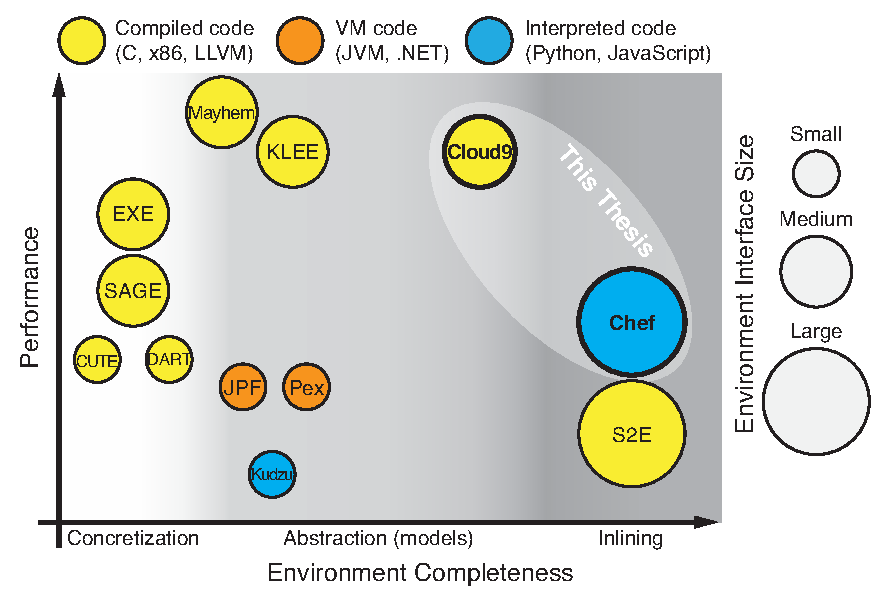
\includegraphics[width=0.8\textwidth]{relatedwork/figures/relwork-positioning}
  \caption{Qualitative comparison of most important symbolic execution engines with respect to the environment problem. X axis indicates completeness of symbolic environment, ranging from no symbolic support (concretization) to full environment inlining.  Y axis indicates relative performance of engines in terms of paths throughput, as deduced from each engine's evaluation numbers.}
  \label{fig:relwork:positioning}
\end{figure}

To efficiently handle real-world programs, symbolic execution engines need to minimize the time spent in the environment, while ensuring correct behavior in the program.
%
Existing approaches roughly fall into three categories, according to the degree of completeness in handling symbolic data going to the environment: (1) concretizing the calls to the environment (no symbolic support at all), (2) abstracting away the environment complexity through models, and (3) ``inlining'' the environment with the program.

Figure~\ref{fig:relwork:positioning} positions the existing work with respect to this classification, while qualitatively indicating the size of the environment interface targeted by the engine and the relative performance attained by each engine in its class.
%
There are several patterns emerging from this classification.

First, the less complete the environment support, the higher the engine performance tends to be.
%
A simpler environment creates fewer execution paths and leads to simpler symbolic expressions in the program state.  In turn, the path throughput in the target program increases.
%
This effect is most visible in symbolic execution engines that resort to concretization or employ simple models, such as EXE~\cite{exe}, Mayhem~\cite{mayhem}, or KLEE~\cite{klee}.

Second, the completeness of the environment tends to be proportional to the complexity of the environment interface of the programs targeted.
%
For example, S2E~\cite{s2eSystem} executes device drivers together with the kernel, as modeling the latter would incur a significant engineering effort.

Third, the engine performance at a given environment completeness level (a vertical in Figure~\ref{fig:relwork:positioning}) depends on the targeted language and the constraint solver performance.
%
Engines targeting compiled code (e.g., KLEE~\cite{klee} or SAGE~\cite{godefroid:fuzz}) are typically faster than engines targeting high-level code (e.g., Kudzu~\cite{saxena-kudzu} or Java PathFinder~\cite{jpf-symbex}).
%
Similarly, newer engines that rely on faster solvers (e.g., EXE~\cite{exe}, SAGE~\cite{godefroid:fuzz}, or KLEE~\cite{klee}) fare better than the early engines (e.g., DART~\cite{dart} or CUTE~\cite{cute}).

Finally, Figure~\ref{fig:relwork:positioning} shows that symbolic execution engines make a \emph{trade-off} between the completeness of their environment and the performance they are willing to sacrifice.
%
From this perspective, our contributions, embodied in the \chef and \cnine symbolic execution engines, advance the state of the art by improving this tradeoff.
%
\cnine retains the performance of model-based environment handling, while providing an accurate operating system model that comes closer in completeness to an inlined approach.
%
\chef benefits from the completeness of inlining the environment---the language interpreter---with the interpreted program, while significantly improving performance over na\"{\i}ve symbolic execution.

In the rest of this section, we discuss in more detail each of the three environment approaches.
%
We use the program in Figure~\ref{fig:relwork:example} as a running example to illustrate the tradeoffs made by each approach.
%
The program opens a file using a symbolic name, reads data from it, then closes it and terminates.  Despite being simple, this example exposes the challenges of the environment problem.

\begin{figure}
  \centering
  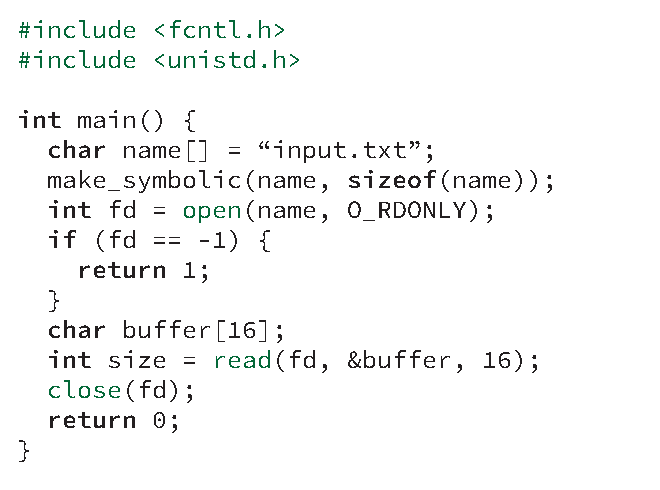
\includegraphics[width=0.6\textwidth]{relatedwork/figures/environment-example}
  \caption{Example of C program using the POSIX operating system interface to open and read a file with a symbolic name.}
  \label{fig:relwork:example}
\end{figure}

\subsection{Under-approximation (Concretization)}

A simple approach to reducing the time spent in the environment is to concretize the values that cross the program boundary~\cite{dart,godefroid:fuzz,klee,exe}.
%
For instance, when the symbolic file name, say $\mu$, is passed as an argument to the \codebit{open} call in Figure~\ref{fig:relwork:example}, the symbolic execution engine replaces the argument with a concrete example $m$.  This causes the execution to proceed linearly inside the environment.

%% For simple programs with limited interactions with their environment, this approach is sufficient.  However, for programs with stronger connections to the environment---e.g., maintaining open file descriptors---concretization may cause missed feasible paths and inconsistencies.

For programs that only send output to the environment (e.g., by calling \codebit{printf}), concretization works well.
%
However, for programs that share state with the environment (e.g., maintain open file descriptors), concretization causes missed feasible paths later in the program execution, or introduces inconsistencies in the program state.

We illustrate these points on our example in Figure~\ref{fig:relwork:example}.
%
First, the returned file descriptor of the concretized \codebit{open} system call is concrete, which causes the symbolic execution engine to exercise only one of the two possible outcomes---success or failure.
%
Second, in order to maintain soundness, concretization introduces constraints in the path condition, which bind the symbolic arguments to concrete examples (in our case, $pc_{new} := pc_{old} \wedge (\mu = m)$).
%
This means the symbolic file name becomes concrete for the rest of the execution path, precluding any symbolic branching on its value.
%
Avoiding the extra constraint in the path condition would keep the file name symbolic, but introduces inconsistency in the program state: while the file descriptor returned by \codebit{open} is \emph{either} valid or failed, the unconstrained symbolic file name would represent \emph{both} valid and invalid file names.
%
This may lead to test cases that increase the coverage in the program, at the expense of also introducing false positives, which manifest as duplicate test cases.

A concrete environment may also introduce inconsistencies if it is shared among all execution paths~\cite{klee}.
%
This is commonly the case with non-concolic (``purely-symbolic'') execution, when the symbolic execution engine maintains all execution states as data structures in its address space.  Calls to the environment would then be passed on to the environment of the engine itself, potentially causing cross-talking between different execution paths.

\subsection{Abstraction (Modeling)}

An alternative approach to simplifying the environment is to replace its concrete implementation with a simpler one---a model---that captures its essential behavior~\cite{klee,mayhem,aeg}.
%
In our running example, a model of the \codebit{open} and \codebit{read} system calls should capture only the two traits used by the program: the ability to read data from the file and the failure when the file is not found.
%
The former can be modeled as an in-memory buffer that is allocated when the file is open and copied to the user buffer in the \codebit{read} system call.
%
The latter can be simulated in the model by branching the symbolic execution state and returning $-1$ in one path.
%
For larger and more realistic programs, an accurate and complete model is significantly larger.  Nonetheness, a model is still smaller than the original implementation---often by orders of magnitude~\cite{klee}---as it drops non-functional requirements, such as performance and fault tolerance.

\paragraph{Executable Models}

The example model we described is \emph{executable code} that runs together with the target program inside the symbolic execution engine, as guest code~\cite{klee}.
%
This approach benefits from the features available in the symbolic execution runtime.  The model can directly access the program state, such as reading and manipulating call arguments using their native types, and directly returning values to the program.
%
In addition, symbolic data implicitly flows through the model code.  The file model in our example implicitly accepts symbolic file names in the \codebit{name} argument of the \codebit{open} system call.

However, some environment features are expensive to capture at the guest level, such as complex control flow abstractions like interrupts and concurrency.
%
In those cases, symbolic execution engines provide models that are built into the engine implementation itself.  For example, the S2E platform~\cite{s2eSystem} provides models for symbolic hardware as built-in platform plugins.
%
Despite their generality, built-in models are harder to write, since they explicitly handle the symbolic program state.

\paragraph{Functional Models}

Models may not only be executable, but also functional, expressed as predicates~\cite{slam-project,klover} or abstract types with theories~\cite{cutie-py,saxena-kudzu,klover}.
%
For instance, the model of a function can be provided as a function summary, consisting of pre-condition and post-condition predicates over the program state~\cite{klover,slam-project}.
In our running example, the summary of the \codebit{open} system call could be $(\mathit{fd} = -1) \vee (\mathit{fd} \geq 3)$.
%
Function summaries may be more efficient than executable code, as they avoid branching the program state and result in more concise symbolic expressions.

Another form of functional modeling is to treat the environment calls as uninterpreted functions~\cite{cutie-py,saxena-kudzu}.
%
The idea is to \emph{lazily} record each environment call as an opaque operation during execution, and provide a decision procedure that interprets the operation at constraint solving time.
%
A benefit of this approach is that specialized decision procedures may be significantly more efficient than executing symbolically the environment implementation.  For example, symbolic execution of web applications~\cite{saxena-kudzu,symjs,jalangi} benefits from constraint solvers that support strings~\cite{Z3,hampi,z3-str,s3-str}, as strings are ubiquitous in this domain.
%
Another benefit is that the interpretation step may end up being skipped if the function call is not relevant for satisfiability~\cite{cutie-py}, as opposed to an executable model, which would be executed regardless of whether the results are used or not.

\paragraph{}

Although they are effective at reducing path explosion, models are expensive to write correctly and completely.  As a result, they tend to be employed only for simple or stable environment semantics, or when the model accuracy is less important (e.g., security testing~\cite{aeg}).

%% \cnine takes the modeling approach to the environment problem, when symbolically executing programs interacting with the operating system.  \cnine is the first to provide an accurate and efficient model for an operating system interface as complex as POSIX.  Key to our approach is to divide the model code into built-in core primitives and guest code, which helps keep the implementation simple, while covering much of the most common operating system abstractions.

\subsection{Inlining (Whole-system Analysis)}

Concretizing environment calls or writing models is unfeasible when the environment interface is large or maintains a complex state, strongly coupled to the program state.
%
For example, once loaded, a device driver typically can interact with the entire operating system kernel.  Concretizing all kernel calls would drastically reduce the exploration space, while modeling all kernel features would be expensive, especially for kernels whose internals change often, such as Linux.

For these cases, an approach that preserves correctness and completeness is to bundle the environment with the program and execute it symbolically as one target.
%
Full-VM symbolic execution engines implicitly provide this approach~\cite{s2e,bitBlaze}.
%
For symbolic execution engines that execute programs in isolation~\cite{klee,godefroid:fuzz}, the environment is explicitly compiled in the target format and linked with the program.

However, this approach reduces the effectiveness of symbolic execution on the original target program, due to the path explosion in the entire system, which may be orders of magnitude larger than the program.
%
Existing work employs several techniques to mitigate path explosion in the environment.
%
For example, S2E~\cite{s2e} introduces execution consistency models, which are principles of converting between symbolic and concrete values when crossing the program boundaries, in order to control the path explosion in the environment.

Another approach is to manually or automatically change the environment implementation to reduce its complexity.
%
For example, the KLOVER symbolic execution engine for C++ programs~\cite{klover} alters the implementation of the \codebit{std::string} STL class to avoid branching inside operators such as equality.
%
In general, the environment code can also be automatically compiled in a form sensible to symbolic execution~\cite{overify}.

%% \chef takes the inlining approach to the environment problem, when symbolically executing programs written in interpreted languages.  \chef is the first system to use a language interpreter as a semantics provider for symbolic execution.


\subsection{Developer Control of Symbolic Environments}

The developer interface to a symbolic execution engine plays an important role in controlling its effectiveness and efficiency.
%
The best known sources of developer inputs are the search selection strategies and the injection of symbolic data in the system.
%
For example, KLEE runs command-line utilities with symbolic arguments defined using a special syntax, in line with the rest of the target arguments.  For instance, \codebit{ls -l --sym-arg 1 3} runs \codebit{ls} with the second argument set as symbolic, between 1 and 3 characters.  This syntax can be used to define symbolic arguments or symbolic files.

The developer control over the symbolic input was encapsulated in concepts such as parameterized unit tests~\cite{tillmann-puts}, which extend regular unit tests with parameters marked as symbolic inputs during symbolic execution.
%
Similarly, QuickCheck~\cite{quickcheck} allows writing input specifications in Haskell, which are used to instantiate inputs during random testing.

%% However, systems software is influenced by many other external factors, such as environment variables, system call failures, thread schedules, signal dispatch timing, and so on.
%% %
%% To address this problem, \cnine's symbolic test interface gives extensive control over the behavior of its operating system model, such as per-file descriptor symbolic fault injection or per-socket symbolic control flow.

%%% Local Variables: 
%%% mode: latex
%%% eval: (visual-line-mode)
%%% fill-column: 1000000
%%% TeX-master: "main"
%%% End:
